\documentclass[11pt]{article}
\usepackage[margin =1in]{geometry}
\usepackage{authblk}
\usepackage{multicol}
\usepackage{graphicx}
\usepackage{subcaption}
\usepackage{xcolor}
\usepackage{float}
\usepackage[hidelinks]{hyperref}
\usepackage{csquotes}
\MakeOuterQuote{"}
\usepackage{amsmath}
\usepackage[backend = bibtex, style = nature, sorting = ynt]{biblatex}
\addbibresource{reference.bib}
\title{{\bf Computational Methods for RNA Secondary Structure Prediction}}
\author[1]{Harrison LaBollita}
\author[2]{Petr \u Sulc}
\date{}
\affil[1]{Department of Physics, Arizona State University, Tempe, AZ 85281 USA}
\affil[2]{Center for Biological Physics, Arizona State University, Tempe, AZ 85281 USA}

\begin{document}

\maketitle
\begin{abstract}
RNA is fundamental to all of life. Much of the biological function of an RNA molecule is given by its secondary structure. In this report, we explore to different computational techniques for RNA secondary structure prediction. We used a convolutional neural network to predict the secondary structure of an RNA molecule. We found that it is limited in its accuracy, because it lacks physical insights. Secondly, we implemented a stem level Gillespie algorithm to predict RNA secondary structures. Our algorithm under-performed compared to leading programs, such as, \texttt{ViennaRNA}. Therefore, there is still room for improvement for our algorithm.  
\end{abstract}
\tableofcontents
\newpage 

\section{Introduction}
\begin{multicols}{2}
RNA is fundamental to all living organisms. It's role in many biological processes is determined by its secondary structure. Therefore, it is critical for biological researchers to gain the capability to accurately predict how a RNA molecule will fold into its secondary structure. This key problem is truly an interdisciplinary one and has required insights from a variety of scientific fields from biology and chemistry to physics and computer science. 

The most successful RNA folder was implemented by Zucker et. al \cite{ZUKER1984591} in the 1980's. Because RNA kinetic folding is a thermodynamic process, it works by via the minimization of free energy. However, many physical systems, such as RNA secondary structures, do not end up in the lowest free energy state. Since Zucker's pioneering algorithm there has been little improvement in predictive accuracy. While Zucker's program is the leading the field, it omits all pseudoknotted secondary structures. However, this means that this program can only predict a pseudoknot free secondary structure. A pseudoknot free structure is simply one that contains no pseudoknotted pairings. A pseudoknot is defined as a secondary structure $S$ with a set of base pairs $(i, j), (k, \ell) \in S$ that satisfies the inequality $i< j < k < \ell$. We have shown a pseudoknotted secondary structure in Figure \ref{fig:pseudo}. Omitting pseudoknotted secondary structure greatly reduces the complexity of the folding problem. An RNA molecule folding into pseudoknot free secondary structure was shown to be solvable in subcubic time by Bringeman et. al \cite{BringmannGSW17}. However, the problem becomes NP-complete if we allow for pseudoknot secondary structures. Pseudoknot secondary structures are of great interest because they offer advantageous functions for applications in biotechnology and nanotechnology \textcolor{red}{Need a citation here or possible examples}. Therefore, there is significant room for improvement in RNA secondary structure prediction with pseudoknots.

In this work, we aim to explore machine learning (ML) techniques for RNA secondary structure by pushing the limits of how far pure ML can go with predicting secondary structures. In addition, we have developed a "proof of concept" stem level Gillespie algorithm for predicting RNA secondary structures with pseudoknot secondary structures.

The remainder of this report is organized as follows: Section 2 describes the data set we used for our ML exploration and the data set we to benchmark the performance of our algorithm. In Section 3, we describe our implementation of a convolutional neural network for RNA secondary structure prediction and the results from our model. In Section 4, we describe our stem level Gillespie algorithm and the benchmark results. Finally, in Section 5, we conclude the report. 
\end{multicols}

\begin{figure}[H]
    \centering
    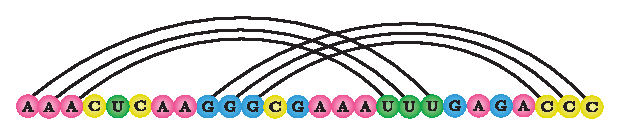
\includegraphics[width = \textwidth]{fig/pseudoknot.eps}
    \caption{Here is an example of a pseudoknotted secondary structure, where we have a crossing of base pairings. A pseudoknot free secondary structure would not have any of the crossing lines in the figure.}
    \label{fig:pseudo}
\end{figure}


\begin{multicols}{2}
\section{Data sets}
We used three independent data sets to benchmark the performance of our CNN and Gillespie algorithm, respectively. The data set we used to train, validate and test our CNN contained over 50,000 RNA sequences all of the length 30 nucleotides (ntds). This data set was generated using NUPACK software \cite{doi:10.1002/jcc.21596}. While it is desirable for CNN to function with variable length sequences, to benchmark performance of our model it was sufficient to use homogeneous length sequences.

For our CNN model, we must encode the sequence and dotbracket information in such a way for the computer to understand it. The sequences are transformed into a matrix, which is described in more detail in a later section. The dotbracket representation is also transformed into a $N \times 3$ matrix, where $N$ is the number of ntds in the sequence and the three columns represent '(', ')', or '.'. A $1$ is placed in the appropriate representation and $0$'s are placed in the remaining columns. For example, if the dot bracket representation of the secondary structure was '((..))', then we would encode this information in the following matrix:
\begin{center}
{\bf ((..))} \hspace{0.1cm} $ \rightarrow$ \hspace{0.1cm}
\begin{tabular}{|c|c|c|}
\hline
1 & 0 & 0\\
1 & 0 & 0\\
0 & 0 & 1\\
0 & 0 & 1\\
0 & 1 & 0\\
0 & 1 & 0\\
\end{tabular}

\end{center}

We created a second data set from the \href{https://rfam.xfam.org}{Rfam database}   which is an online collection of thousands of RNA families that contain the sequence, secondary structure, and the free energy of the secondary structure \cite{ 10.1093/nar/gkv480, doi:10.1002/cpbi.51}. This data set contains 27 sequences with variable lengths. The complete data set statistics are contained in Figure \ref{fig:rfam}.

Finally, our third data set was created \href{http://pseudobaseplusplus.utep.edu/home}{Pseudobase} another online database of RNA sequences, but these contain only pseudoknotted secondary structures \cite{10.1093/nar/28.1.201}. This data set contains 15 sequences with variable lengths. We have provided the data set statistics in Figure \ref{fig:pseudobase}.

In a later section, we provide our benchmark results of our stem level Gillespie algorithm compared \texttt{ViennaRNA} \cite{Lorenz2011}, a well-known program for RNA secondary structure prediction.
\end{multicols}

\begin{multicols}{2}
\begin{figure}[H]
\centering
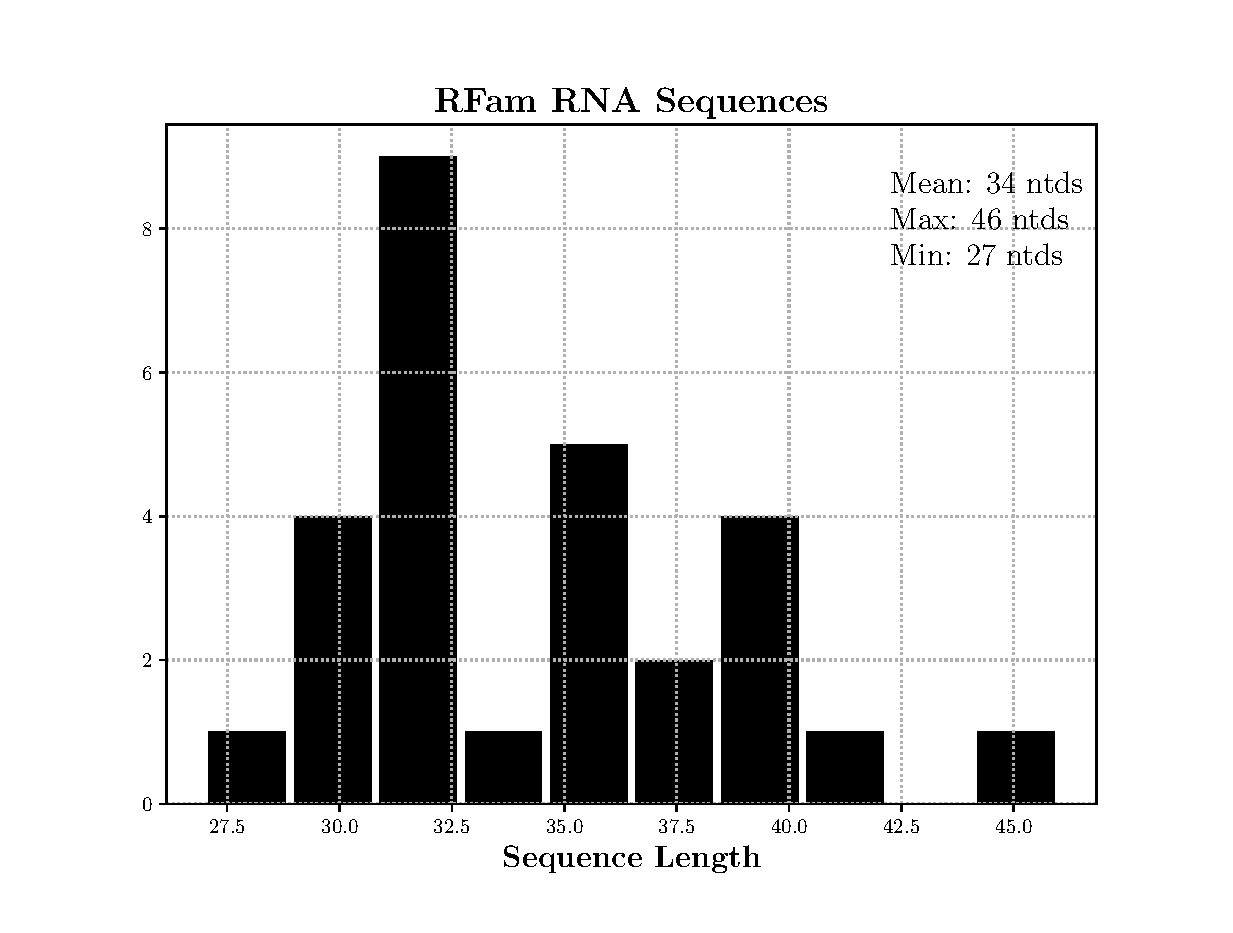
\includegraphics[width = 0.5\textwidth]{fig/rfam}
\caption{The Rfam data set contains 27 total sequences with variable length. The average length is 34 ntds. The longest sequences is 46 ntds and the shortest sequence is 27 ntds.}
\label{fig:rfam}
\end{figure}

\begin{figure}[H]
    \centering
    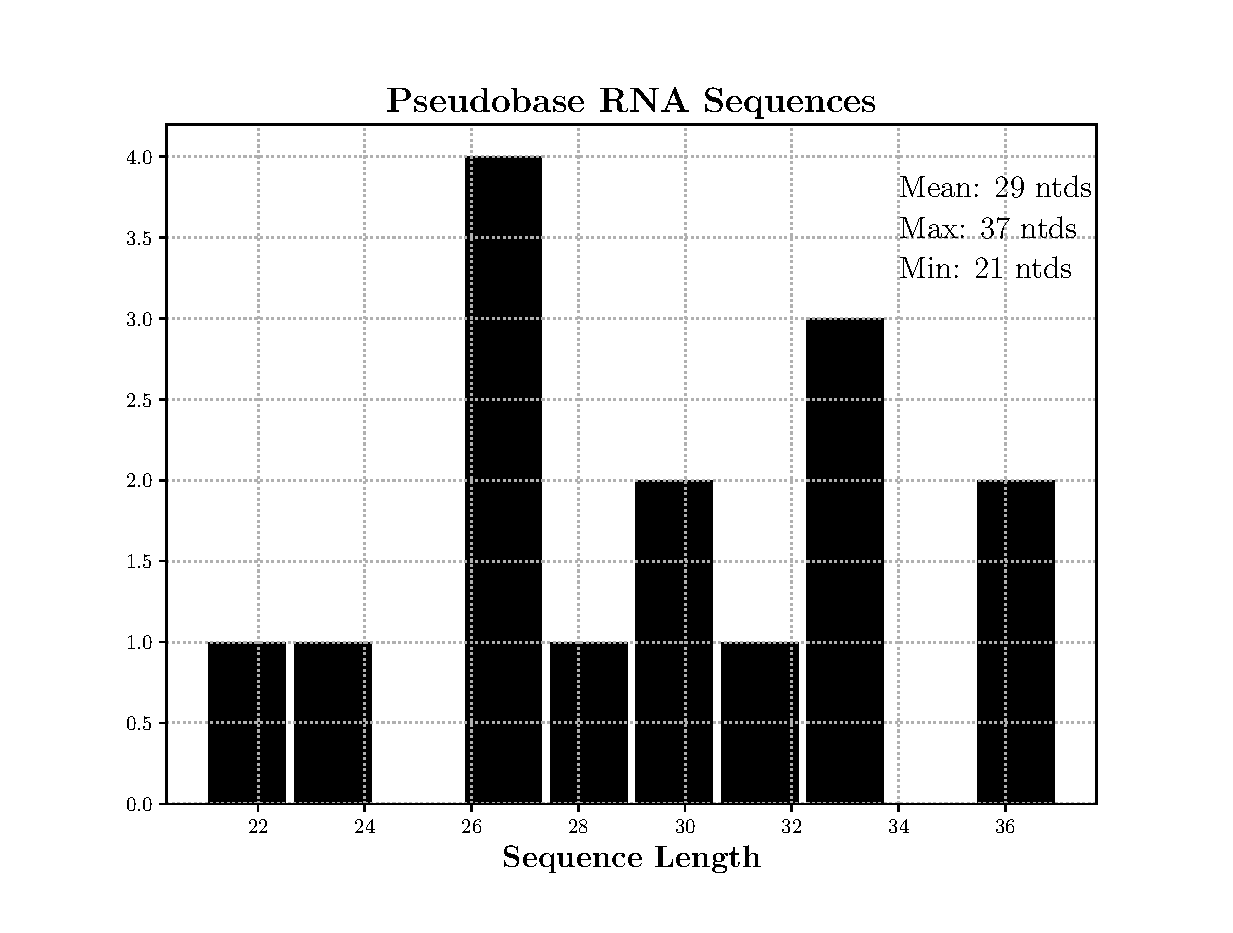
\includegraphics[width = 0.5\textwidth]{fig/pseudobase.eps}
    \caption{The Pseudobase data set contains 15 total sequences with variable length. The average length is 30 ntds with a maximum length sequence of 38 ntds and minimum length of 22 ntds.}
    \label{fig:pseudobase}
\end{figure}
\end{multicols}

\begin{multicols}{2}
\section{CNN Predicts Secondary Structure}
Convolutional neural networks (CNN)s are machine learning algorithms that are primarily used for image classification problems. The input layer is the image’s RGB values, which are then fed through multiple convolution layers, that are finally connected to a standard fully-connected feed forward neural network. Ultimately, to use a CNN one must have data that can be interrupted as an image. Following \cite{10.3389/fgene.2019.00467}, we have replicated their CNN in PyTorch \cite{paszke2017automatic} in efforts to achieve similar results.


\subsection{Matrix Representation of RNA}

RNA sequences are comprised of any combination of four nucleotide bases: adenine (A), guanine (G), cytosine (C), and uracil (U). When using ML techniques for RNA secondary structure prediction, a formidable challenge is how to encode the sequence as input for the ML architecture. We have chosen to encode the sequence as a matrix in order to use a CNN architecture. The rules of folding a RNA secondary structure are very simple: A pairs with U, G pairs with C, and sometimes G pairs with C. The canonical pairs A-U and G-C are called Watson-Crick pairs \cite{Cleaves2011}, while the G-U pair is known as the wobble pair. Following these simple rules, we can build a weighted matrix based on which base is more likely to pair with whom. The complete matrix building algorithm is explain in \cite{10.3389/fgene.2019.00467}, and our source code is available on this \href{https://github.com/harrisonlabollita/RNA-ML/blob/master/src/explore/cnn%20code/rna2matrix.py}{GitHub repository}.

\subsection{Model}

The architecture of our CNN is simple. The  model contains two convolutional layers, two pooling layers, and three fully-connected layers. We use a binary cross-entropy loss function, since we are predicting either a value of 0 or 1. We optimized the hyperparameters in our model via configuration space searching, where we randomly choose parameters from our configuration space, train our network and log the performance. We found that a learning rate of 0.001 and momentum of 0.9 performed the best without over-fitting.

We have illustrated the workflow of our CNN Model in Figure \ref{fig:cnn_model}. We begin with an RNA sequence, convert the sequence into a matrix, then feed it into our CNN. The output of the CNN is a $N \times 3$ matrix, where $N$ is the number of nucleotides in the sequence and our model's predicted values of each nucleotide being paired or unpaired. From this information, we reconstruct the dotbracket representation by choosing the highest value in each row as the model's choice for paired ("(" or ")") or unpaired (".") and compare our predicted structure with the actual secondary structure for this sequence.
\end{multicols}

\begin{figure}[H]
\centering
\hspace*{-8cm}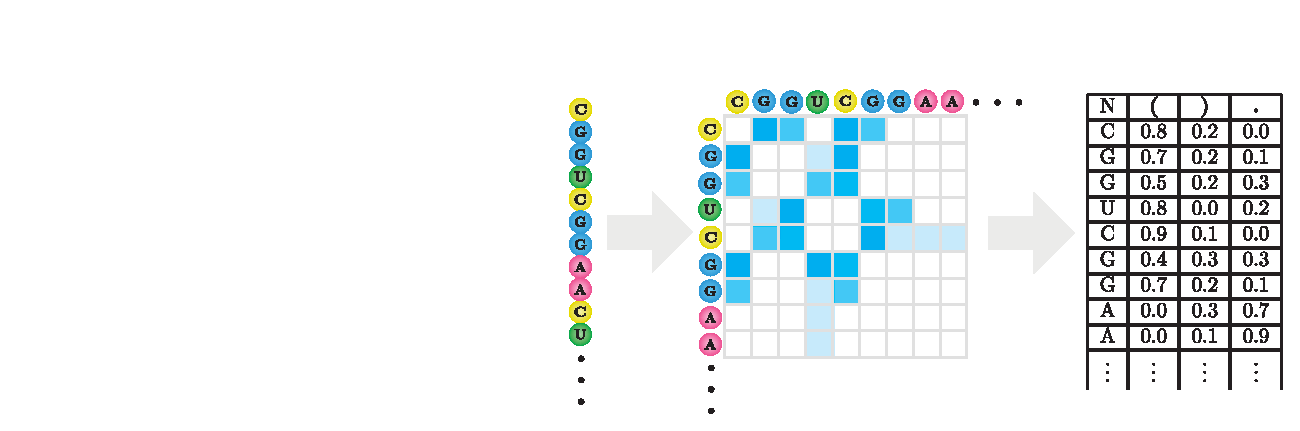
\includegraphics{fig/cnn_model_outline}
\caption{We convert our data set of RNA sequences into a new data set of RNA matrices. These matrices are used as inputs into our CNN. Notice that the darker blue squares correspond to heavier weighted base meaning more likely to be paired. The output of our network is the matrix on the far right which we use to reconstruct the dot bracket representation of the secondary structure.}
\label{fig:cnn_model}
\end{figure}

\begin{multicols}{2}
We trained and validated our CNN model on data set containing 50,000 uniform length RNA sequences following the standard condition, where 80\% of the data is used for training and 20\% of the data set was used for validation. We trained our network for 100 epochs with a batch size of 100. We quantified the accuracy of our model by counting the number of mistakes our model made when predicting the secondary structure. A perfect prediction corresponds to 0 mistakes.
\end{multicols}

\begin{multicols}{2}
\subsection{Results and Discussion}
In this section, we present our CNN model's performance on RNA secondary structure prediction. In Figure \ref{fig:acc}, we have plotted the training and validation accuracy of our model throughout the training session. We can see that the model converges to about 84\% accuracy for both training and validation accuracies.

Our CNN model achieves similar results to the \cite{10.3389/fgene.2019.00467}, however, our model will sometimes predict non-physical structures. Therefore, it is necessary that we include a dynamic layer in our model that corrects for these non-physical outputs. This is the central weakness of all non-physical secondary structure predictors. Without including knowledge of physical considerations these models will always produce un-physical secondary structures.

\end{multicols}

\begin{figure}[H]
\centering
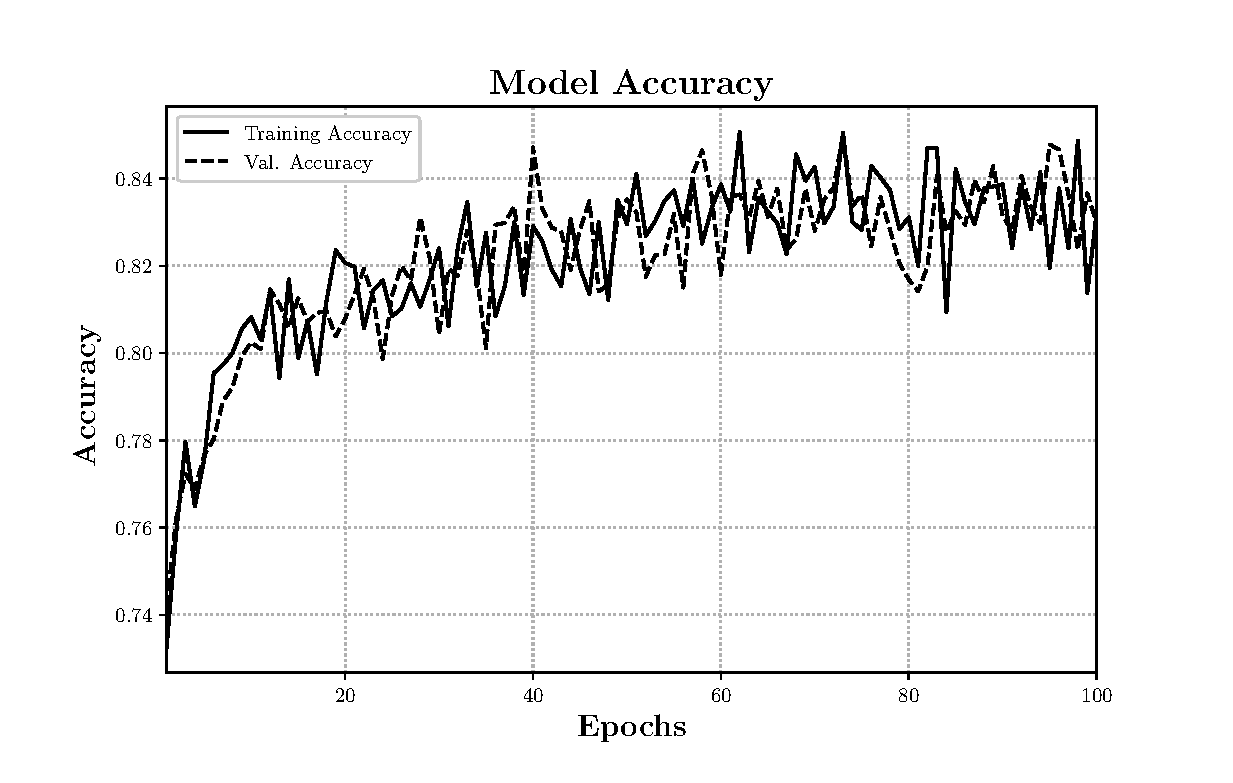
\includegraphics[width = \textwidth]{fig/acc}
\caption{Training and validation accuracy over the 100 epochs. The solid black line is the training accuracy and the dotted black line is the validation accuracy.}
\label{fig:acc}
\end{figure}

\begin{figure}[H]
\centering
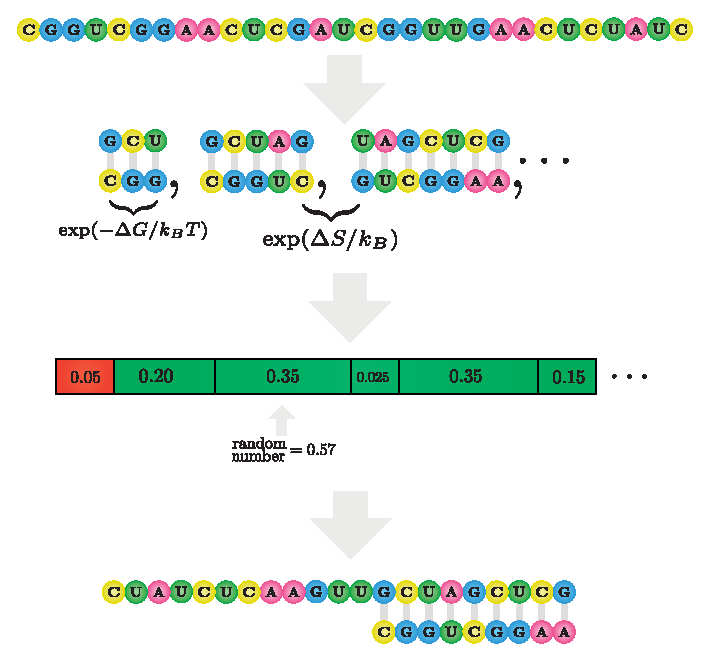
\includegraphics[scale = 1.1]{fig/rna_gillespie_algo}
\caption{Above is an illustration of our algorithm. We begin with a open strand sequence. From here we generate a move set of all possible moves, in this case, all the possible stems that could form. We assign a transition rate from the current state $S_{i}$ to the next state $S_{j}$. We then stochastically choose a move to happen from our probability distribution. We propagate our structure to this next move, then regenerate a move set with new transition rates. We continue to do this until we have reached our maximum running time. The result is our folded structure. }
\label{fig:gill_algo}
\end{figure}
\begin{multicols}{2}
\section{Stem Level Gillespie Algorithm}

\subsection{Stem Level Implementation}
There are two central approaches when writing a computer program to simulate RNA folding kinetics: base pairs or stems. The first approach considers the transitions from RNA states at the base pair level, which generates a microscopic picture of the RNA folding events \cite{10.1093/nar/gkv480}. The alternative approach is to consider large arrangements of base pairs or stems. The transition between RNA states is then completed via forming or breaking a complete stem rather than single base pairs. In this work, we propose a Gillespie algorithm that works at the stem level. We intend for the algorithm to be used for long RNA stands ($>$ 100+ ntds), therefore, the stem level implementation is computationally more desirable than working at the base pair level.

As mentioned above we implement a Gillespie algorithm, which is a stochastic simulation algorithm to perform our RNA folding kinetics. The Gillespie algorithm is very popular for simulating chemical reactions.  For a more complete discussion of the Gillespie algorithm please see Ref. \cite{erban2007practical}. We will briefly go over our algorithm and additionally, we have provided an illustration of our algorithm in Figure \ref{fig:gill_algo}.

Our algorithm begins by first defining a set of moves and a set of transition rates that correspond to each move. There are two different rates: one for creating a stem, which we calculate from the entropy

\begin{equation}
\text{Rate of forming stem} = \exp \Big (\frac{ \Delta S}{k_{B}} \Big ),
\end{equation}
where $k_{B}$ is the Boltzmann constant in the correct units. The entropy term is the sum loop entropy, bond entropy, and duplex entropy for that state. The rate of breaking is given by

\begin{equation}
\text{Rate of breaking stem} = \exp \Big ( - \frac{ \Delta G}{k_{B} T} \Big ).
\end{equation}

These rates form a probability distribution from which we can stochastically sample from to choose our next move. Upon transitioning from state $S_{i} \rightarrow S_{j}$ to our next state. We regenerate a new move set and re-calculate the transition rates between the current structure state and all other possible structure states. We have include a diagrammatic illustration of our algorithm in Figure \ref{fig:gill_algo}. Referencing the figure, one can see that we begin with a RNA sequence, then find the move set. From here we generate the probability distribution, where the sum of all of the transition rates sum to 1. We generate a random number and find in which been the random number falls. We then choose this move that corresponds to this rate whether it is to break a currently formed stem or form a new stem. We repeat this process until we reach a cutoff time that is set by the user. We experimented with different cutoff times to find a quasi-optimal time to let the algorithm run.
This completes our description of our stem level Gillespie algorithm in the next section we present our results and discussion.
\end{multicols}


\begin{figure}[H]
\begin{small}
\begin{verbatim}
Sequence: CGGUCGGAACUCGAUCGGUUGAACUCUAUC
Time: 0.1945s | Added Stem: [[10, 17], [11, 16]] | Current Structure: ..........((....))............
Time: 4.4331s | Added Stem: [[5, 29], [6, 28]] | Current Structure: .....((...((....))..........))
Time: 4.9914s | Added Stem: [[7, 19], [8, 18]] | Current Structure: .....((((.((....))))........))
Time: 6.2564s | Added Stem: [[1, 24], [2, 23]] | Current Structure: .((..((((.((....))))...))...))
\end{verbatim}
\end{small}
\caption{A sample output from our algorithm.}
\end{figure}

\begin{multicols}{2}
\subsection{Results and Discussion}

In this section, we present and discuss the benchmark results of our stem level Gillespie algorithm and compare them with benchmark results of Vienna RNA program \cite{Lorenz2011}. We tested our algorithm on the second and third data sets mentioned above, which was derived from the Rfam database and Pseudobase database, respectively. Recall both of these data sets consisted of variable length RNA sequences with mean length of about 30 ntds. Also, the data set from Psuedobase contains only sequences with secondary structures that contain pseudoknots.

In order to quantify the performance of our algorithm, we first obtain benchmark results on \texttt{ViennaRNA}'s performance on our data set. We use the results as the baseline for our algorithm's performance. We quantify error as the number of mistakes made in our prediction compared to the known secondary structure. The number of mistakes is then normalized to the length of the RNA sequence.

\subsubsection{Rfam Results}
In Figure \ref{fig:vbench}, we have plotted a histogram of ViennRNA's performance. The histogram shows the percentage of the secondary structure that \texttt{ViennaRNA} predicted incorrectly. We can see that the average error was about $10\%$. The worst prediction was $57\%$ and the best prediction was $0\%$ or $100\%$ correct.

We now use the same data set with the Gillespie algorithm. Again, we have plotted a histogram of our program's performance. We can see from Figure \ref{fig:gill} that on average we predicted $38\%$ of the secondary structure incorrectly. Our best prediction was only $21\%$ incorrect and our worst prediction was $54\%$ incorrect.

\subsubsection{Pseudobase Results}
In Figure \ref{fig:v_pseudo}, we have shown a histogram of \texttt{ViennaRNA}'s performance on the Pseudobase data set. We can see that on average \texttt{ViennaRNA} predicted a secondary structure that was $35\%$ incorrect. The worst prediction by \texttt{ViennaRNA} was $62\%$ incorrect and the best prediction was $23\%$ incorrect.

In Figure \ref{fig:gill_pseudo}, we have shown a histogram of our algorithms performance on the Pseudobase data set. On average our algorithm predicted a secondary structure that was $46\%$ incorrect. The best prediction was $18\%$ incorrect or $82\%$ correct. Our worst prediction was $71\%$ incorrect. 

\end{multicols}

\begin{multicols}{2}
\begin{figure}[H]
\centering
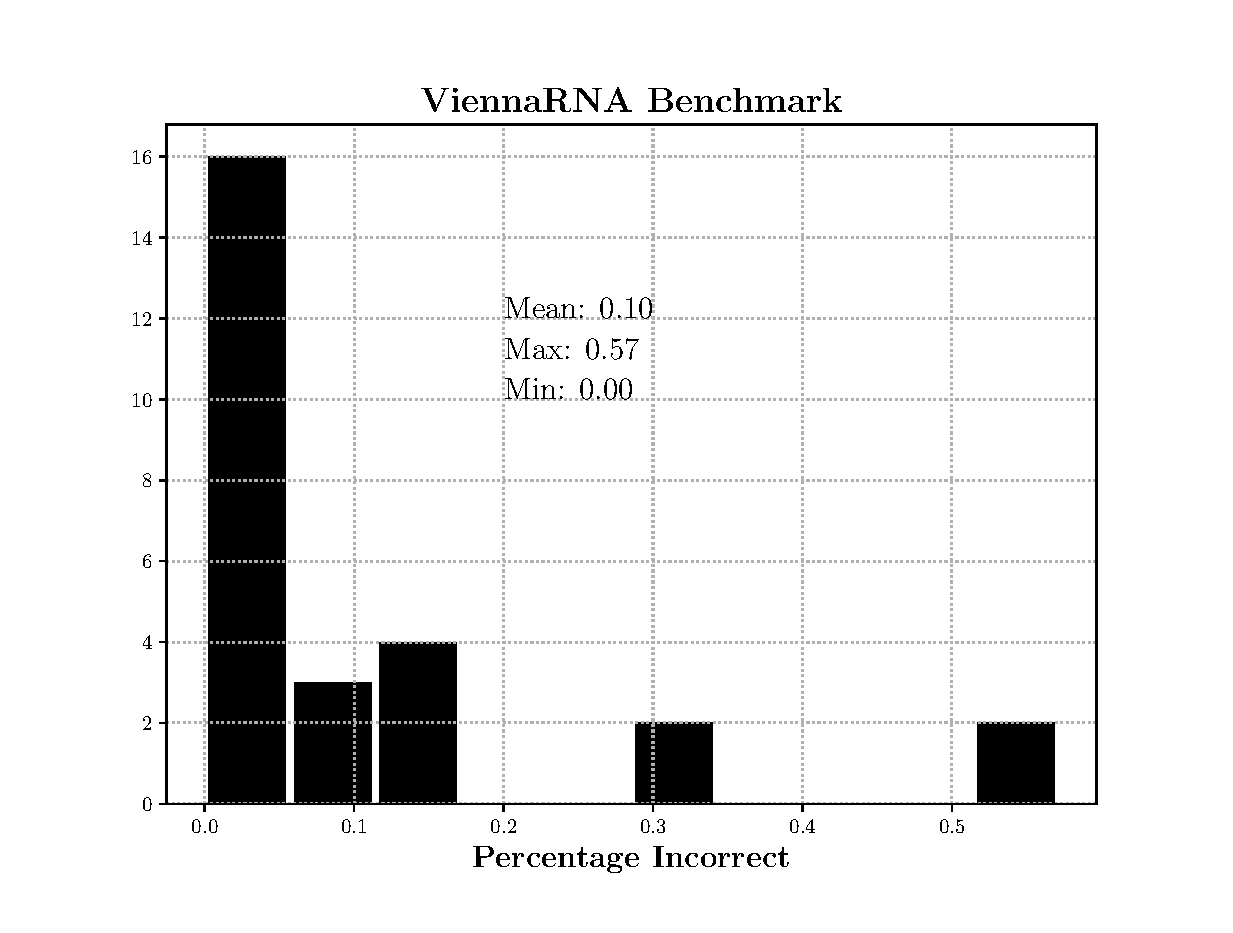
\includegraphics[width = 0.55\textwidth]{fig/v_rna_bench}
\caption{To benchmark our performance, we compared our algorithm to a popular RNA secondary structure predictor Vienna RNA \cite{Lorenz2011}. The $x$-axis is the percentage of the structure that we incorrectly predicted. The mean was $10\%$, the worst prediction was $0.57\%$, and the best prediction was $57\%$. }
\label{fig:vbench}
\end{figure}

\begin{figure}[H]
\centering
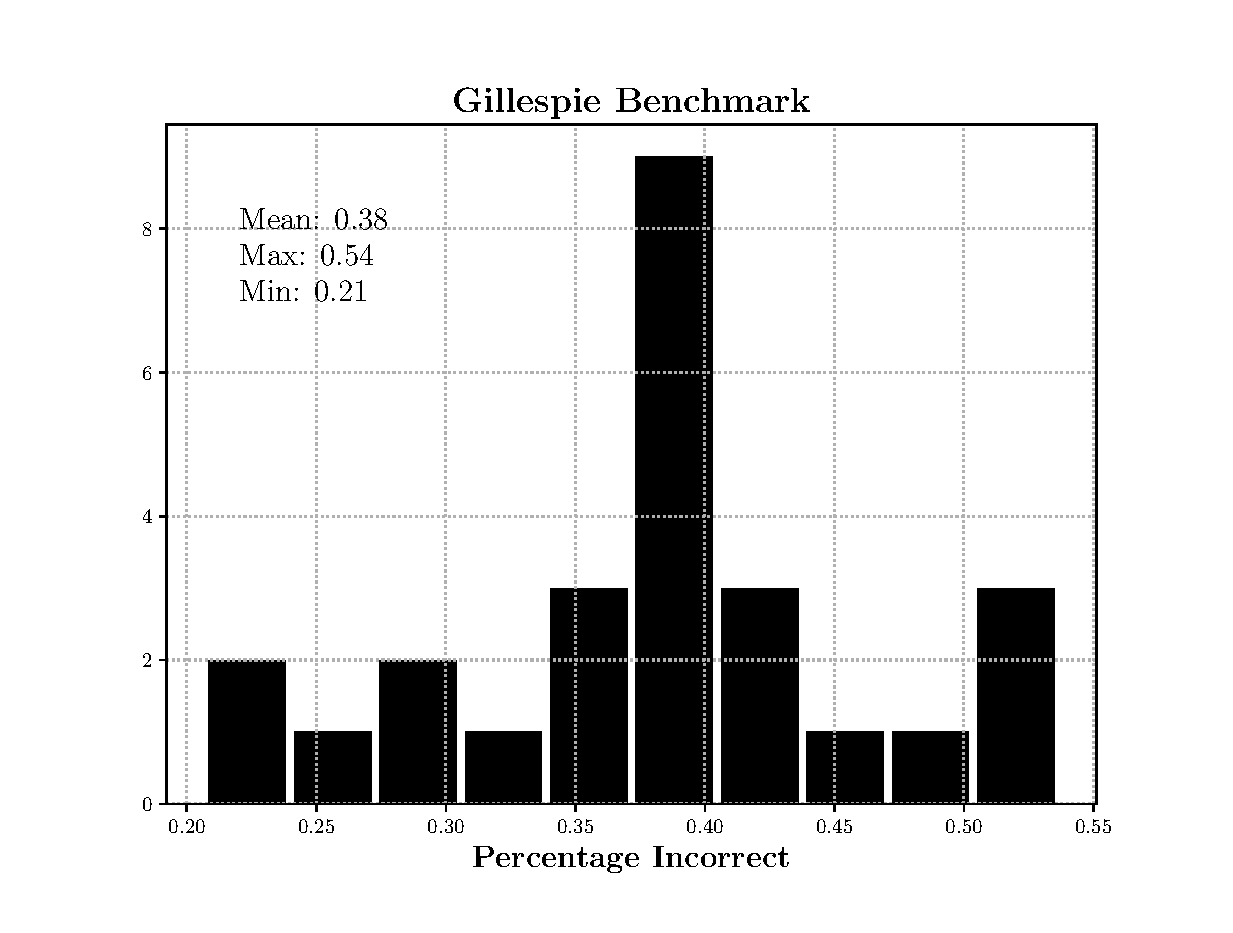
\includegraphics[width = 0.55\textwidth]{fig/gill_bench}
\caption{A histogram of the Gillespie algorithm's performance. The $x$-axis represents the percentage of the structure that was incorrectly predicted by our algorithm. The mean is $38 \%$, the worst prediction  was $54\%$, and the best prediction was $21 \%$.}
\label{fig:gill}
\end{figure}
\end{multicols}

\begin{multicols}{2}
\subsubsection{Discussion}

We can see from Figures \ref{fig:vbench},\ref{fig:gill}, \ref{fig:v_pseudo},\ref{fig:gill_pseudo} that \texttt{ViennaRNA} outperformed our algorithm on both the Rfam and Pseudobase data set. We know that the \texttt{ViennaRNA} never predicted the correct secondary structure for the Pseudobase data set simply because it does not allow for secondary structures with pseudoknots. 

These results indicate that there needs to be various improvements made to our algorithm. We can make various improvements to how the algorithm propagates the folding structure through the state space. In addition, we need to make several adjustments to make the algorithm run computationally faster. Furthermore, we can fine tune certain parameters of the algorithm such as the maximum time it can run to achieve potentially better results.
\end{multicols}
\newpage 

\begin{multicols}{2}
\begin{figure}[H]
    \centering
    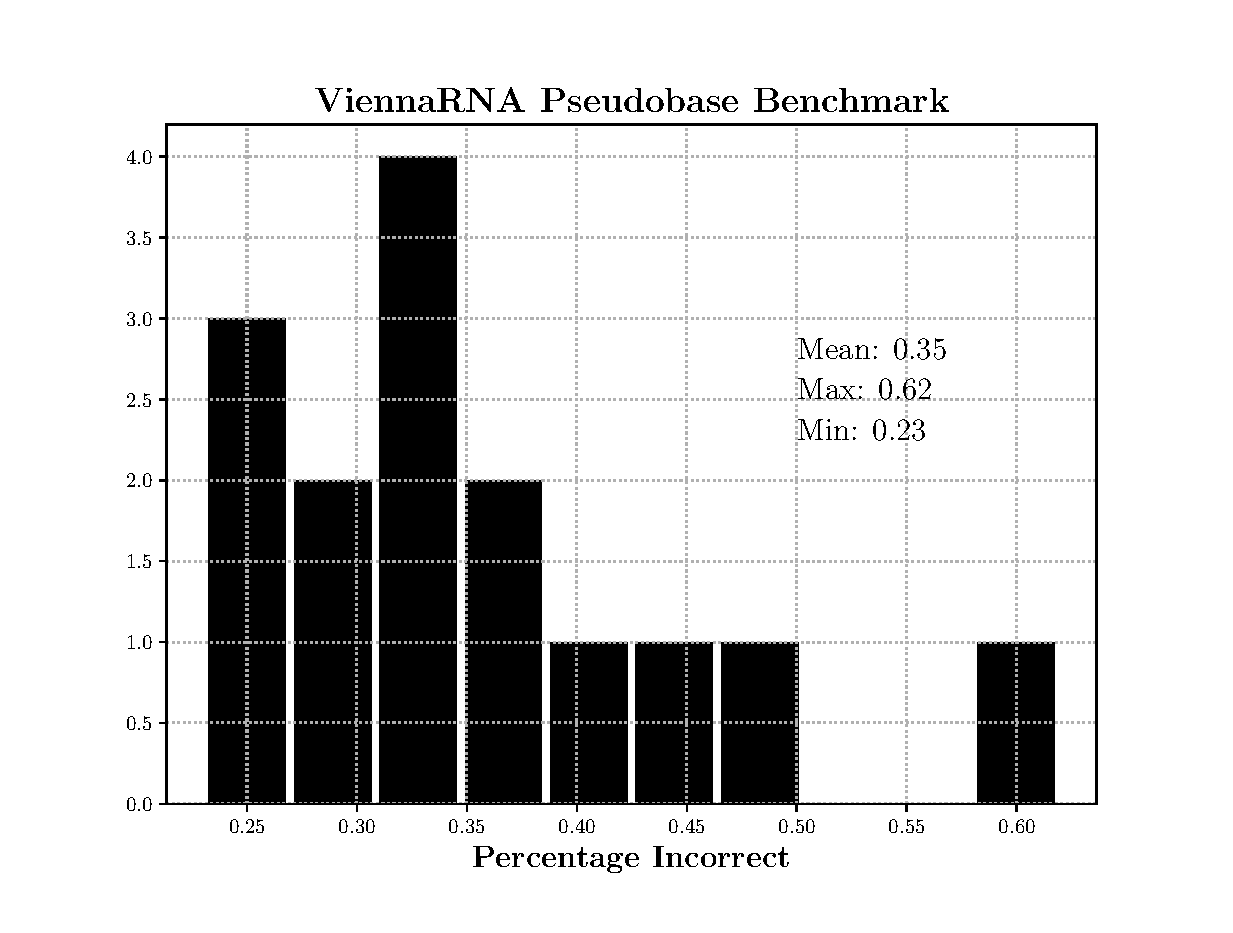
\includegraphics[width = 0.55\textwidth]{fig/v_rna_pseudo.eps}
    \caption{A histogram of \texttt{ViennaRNA}'s performance on the Pseudobase data set. This plot is formatted in the same way as previous histograms shown above. The mean predicted secondary structure was $35\%$ incorrect.}
    \label{fig:v_pseudo}
\end{figure}

\begin{figure}[H]
    \centering 
    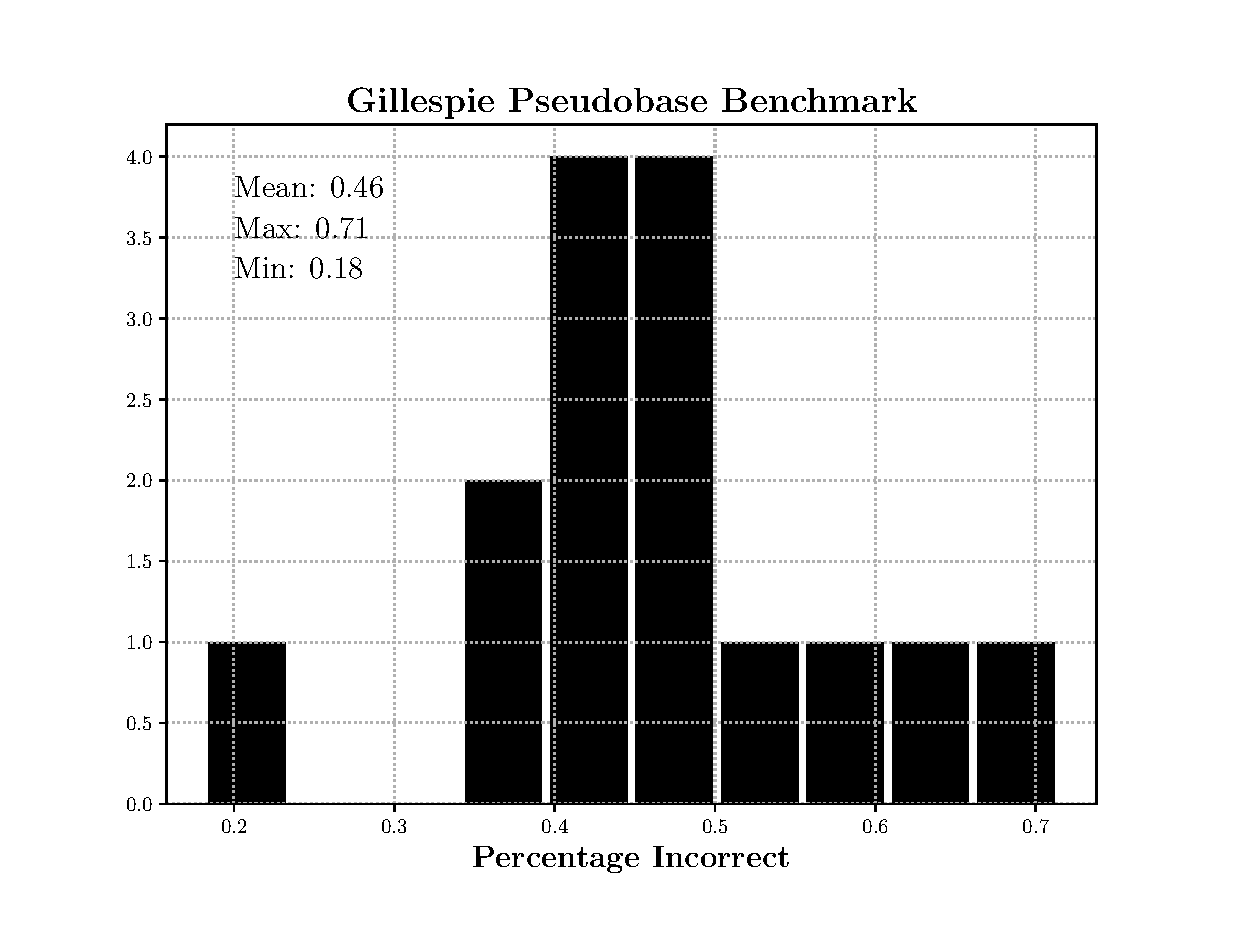
\includegraphics[width = 0.55\textwidth]{fig/gill_pseudo.eps}
    \caption{A histogram of our algorithm's performance on the Pseudobase data set. This plot is formatted in the same way as previous histograms shown above. The mean predicted structure was $46\%$ incorrect.}
    \label{fig:gill_pseudo}
\end{figure}
\end{multicols}

\begin{multicols}{2}
\section{Conclusion}
The secondary structure of an RNA molecule encodes much information about its biological function. Therefore, the ability to predict and understand how a RNA sequence will fold into its secondary structure would unlock many possibilities in biotechnology and nanotechnology. Unfortunately, the general RNA folding problem is NP-complete. 

In this work, we have presented two computational methods to address the folding problem. The first was a CNN that was primarily used to explore the possibilities of ML techniques for RNA folding. We found that ML techniques are quite limited in their performance, because they lack much of the physical insights to the problem given by thermodynamics and statistical physics. 

Our second computational tool to address RNA folding was a stem level Gillespie algorithm, which has the ability to predict secondary structures that contain pseudoknots. We compared our algorithm's performance with a well-known secondary structure prediction program called \texttt{ViennaRNA}. Unfortunately, \texttt{ViennaRNA} outperformed our algorithm on both of our data sets. However, our algorithm is constructed with the capability of predicting to a secondary structure with pseudoknots. Therefore, it is worth refining and adjusting our implementation in the aforementioned ways to hopefully outperform a leading program such as \texttt{ViennaRNA}.

While the RNA folding problem remains unsolved. We have explored two computational methods that could be potentially viable options. We conclude that ML techniques are unlikely to perform better than the current leading algorithms. A more viable solution will most likely emerge from the adaptations physical models designed to minimize the free energy of the secondary structure. 
\end{multicols}

\section*{Acknowledgments}
HL would like to thank Petr \u Sulc for working with on this project to fulfill the requirement of PHY 500 (Research Methods). It has been wonderful exploring and learning about RNA molecules and secondary structure prediction.
\newpage

\nocite{*}
\printbibliography

\end{document}